\documentclass[a4paper, 11pt]{article}
\usepackage[utf8]{inputenc}
\usepackage{comment} % enables the use of multi-line comments (\ifx \fi) 
\usepackage{lipsum} %This package just generates Lorem Ipsum filler text. 
\usepackage{fullpage} % changes the margin
\usepackage{listings}
\usepackage[usenames,dvipsnames]{xcolor}
\def\digitcolor{\color{Magenta!80}}
\usepackage{graphicx}

\begin{document}
%Header-Make sure you update this information!!!!
\noindent
\large\textbf{Disciplina: }Sistemas Operacionais I\\
\normalsize \textbf{Código disciplina: }ESTCMP007 \\
\textbf{Professor: }Maurício Serodio Figueiredo \\
\textbf{Alunos: }Rodrigo da Costa Moraes - 1315208157, Wesley da Silva Rocha - 1715310026 \\
\textbf{Relatório: }\large Trabalho de Threads e Sincronização

% - Introdução
%     - Explicar o que é
%          - processamento paralelo
%          - o que são threads
%          - sincronização das threads
%          - sincronização das threads com semáforos
% - problema produtor/consumidor
% 	- Descrição da Solução do problema produtor/consumidor
% 	- Implementação(deve conter descrição geral do código)
% - problema leitores e escritores
% 	- Descrição da Solução do problema leitores e escritores
% 	- Implementação(deve conter descrição geral do código)
% - Threads em Python 3
%     - Descrição do funcionamento da tarefa
%     - Descrição do funcionamento do código
%     - Código(deve conter descrição geral do código)

\section{Introdução}
A menor sequência de instruções programadas que pode ser gerenciada independentemente pelo Gerenciar de Tarefas(\textit{Scheduler}), é chamado de \textit{Thread}. Devido ao fato de as \textit{Threads} terem a possibilidade de ser gerenciadas independentemente de outras \textit{Threads} e processos, elas são usadas para realizarem processamento em paralelo. E no caso de as \textit{Threads} compartilharem algum recurso em comum, chama-se esse processo de processamento concorrente, onde as \textit{Threads} vão dividir um determinado recurso.

As \textit{Threads} compõem um determinado programa ou processo, e devido a esse não ter uma forma determinada, não é possível paralelizar, não ao menos da forma mais eficiente possível, o programa em várias \textit{Threads}, ficando esta tarefa a cargo do usuário programador. Que deve conhecer o comportamento completo de seu programa, e que assim, pode determinar que partes dos códigos podem ser executadas independentes e que recursos devem ser compartilhados ou não. Sendo assim, o programa deve ser explicitamente programado para o uso de \textit{Threads}.

Visto que o usuário programador é quem determina as \textit{Threads} em que o programa pode ser dividido e que recursos devem ser compartilhados, além disso ele deve informar ao Sistema Operacional como essas \textit{Threads} vão acessar determinado recurso compartilhado, ou seja, quais as restrições de acesso ao recurso para todas as \textit{Threads} do programa, de forma a manter a integridade do funcionamento de seu algoritmo, e também desempenho deste. Visto que o usuário programador também deve conter grande conhecimento do \textit{hardware} em que este programa irá executar, porque isto influenciará diretamente na quantidade de \textit{Threads} utilizadas, bem como restrições de memória.

A esse processo de controle do acesso ao recurso compartilhado e também de troca de informação entre \textit{Threads} e processos, é chamado de Sincronização. Alguns problemas clássicos serão abordados nesse trabalho, como o do Produtor e Consumidor com \textit{buffer} limitado e dos Leitores e Escritores.

\section{Problema: Produtor e Consumidor com \textit{buffer} limitado}
Consiste em um conjunto de processo que compartilham um mesmo \textit{buffer}, que possui tamanho limitado. Os processos chamados de produtores são os responsáveis por inserir informação no \textit{buffer}. Já os processos chamados de consumidores são os responsáveis por remover informações do \textit{buffer}. 

Pode-se observar que entra-se em um empasse, quando um produtor quer inserir um processo no \textit{buffer}, e o consumidor quer remover a informação, contudo, isso acontecendo ao mesmo tempo, o que pode causar inconsistência nas informações, pois, o escritor pode deixar um consumidor com informações desatualizadas.

Problemas relacionados ao \textit{buffer} ser limitado também deve ser tratados, como o produtor não inserir mais informações quando o \textit{buffer} estiver sem espaço vazio, e o consumir não remover do \textit{buffer}, quando este estiver sem espaço preenchido. O que pode vir a causar falha de segmentação.

\subsection{Descrição da Solução}
Para facilitar o desenvolvimento do programa e também o entendimento por terceiro, apelidou-se as funções \textit{sem\_post} e \textit{sem\_wait}, para UP, e DOWN, respectivamente. Onde a função UP realiza a operação de adicionar um no valor semáforo, assim que for possível, e a função DOWN realiza a operação de diminuir um no valor do semáforo, assim que for possível.

Os semáforos utilizados foram \textit{mutex}, semáforo binário, que controla o acesso ao \textit{buffer}; \textit{empty}, que controla o acesso a informação de espaços vazios do \textit{buffer}, \textit{empty\_cnt}; e \textit{filled}, que controla o acesso a informação de espaços preenchidos do \textit{buffer}, \textit{filled\_cnt}.

Para simular o comportamento do \textit{buffer} foi utilizado um vetor caracteres, de tamanho \textit{BUFFER\_MAX}, e com valores de espeço vazio indicados por \textit{BUFFER\_DEFAULT}.

A quantidade produtores é determinada por \textit{PRODUCER\_CNT}, e a de consumidores é determinada por \textit{CONSUMER\_CNT}.

As informações a serem produzidas e consumidas estão em \textit{to\_produce}, que é um vetor de caracteres. Somente um elemento de \textit{to\_produce} é processado por vez, ou seja, o produtor somente um produz um caracter por vez de \textit{to\_produce}, assim como o consumidor somente consome um caracter por vez do \textit{buffer}. \textit{to\_produce\_cnt} contém a próxima informação a ser processada de \textit{to\_produce}.

Para simular um processo real usou-se um atraso após a produção e consumo. E para se ter uma resposta variável, mas determinada, de forma que todo o \textit{buffer} fosse utilizado, foi usada a função \textit{seno} e \textit{cosseno}, com fasor de -90 graus. O resultado segue abaixo.

\begin{figure}[!h]
\caption{Execução do Programa Produtor e Consumidor}
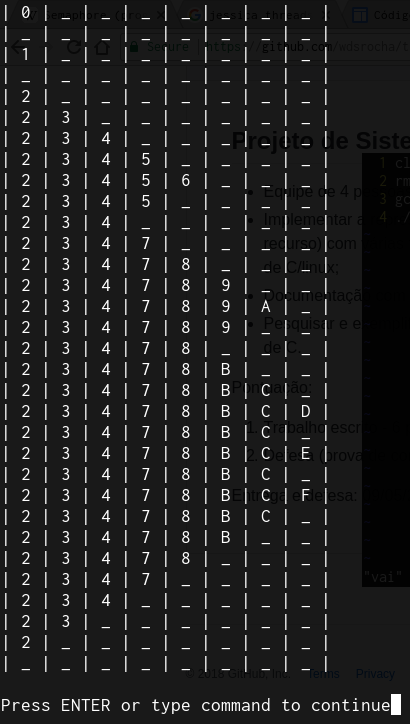
\includegraphics[height=10cm]{produtor_consumidor}
\centering
\label{fig1}
\end{figure}

\lstset{language=C}
\begin{lstlisting}
#include <stdlib.h>
#include <stdio.h>
#include <pthread.h>
#include <semaphore.h>
#include <unistd.h>
#include <math.h>

#define UP(x) sem_post(&x)
#define DOWN(x) sem_wait(&x)

#define BUFFER_DEFAULT '_'
#define BUFFER_MAX 8 

#define PRODUCER_CNT 2

#define CONSUMER_CNT 2

#define TIME_INCREMENT 0.2-M_PI/2.0

pthread_t producer_t, consumer_t;
sem_t mutex, empty, filled;
char buffer[BUFFER_MAX];
char to_produce[] = "0123456789ABCDEF";
int empty_cnt = BUFFER_MAX;
int filled_cnt = 0;
int to_produce_cnt = 0;
int timer = 0;

void *produce();
void *consume();
void bufferInit();
void bufferProduce();
void bufferConsume();
void bufferDisplay();

int main() {
    srand(time(NULL));

    bufferInit();

    sem_init(&mutex, 0, 1);
    sem_init(&empty, 0, BUFFER_MAX);
    sem_init(&filled, 0, 0);

    for (int i = PRODUCER_CNT; i--;) {
        pthread_create(&producer_t, NULL, produce, NULL);
    }

    for (int i = CONSUMER_CNT; i--;) {
        pthread_create(&consumer_t, NULL, consume, NULL);
    }

    for (int i = PRODUCER_CNT; i--;) {
        pthread_join(producer_t, NULL);
    }

    for (int i = CONSUMER_CNT; i--;) {
        pthread_join(consumer_t, NULL);
    }

    return 0;
}

void *produce() {
    while (to_produce[to_produce_cnt] != '\0') {
        DOWN(empty);
        DOWN(mutex);
        bufferProduce();
        UP(filled);
        UP(mutex);

        sleep(1+sin(timer));
        timer += TIME_INCREMENT;
    }
}

void *consume() {
    while (filled_cnt > 0 || to_produce[to_produce_cnt] != '\0' ) {
        DOWN(filled);
        DOWN(mutex);
        bufferConsume();
        UP(empty);
        UP(mutex);

        sleep(1+cos(timer));
        timer += TIME_INCREMENT;
    }
}

void bufferInit() {
    for (int i = 0; i < BUFFER_MAX; i++) {
        buffer[i] = BUFFER_DEFAULT;
    }
}

void bufferProduce() {
    if (empty_cnt > 0) {
        buffer[filled_cnt] = to_produce[to_produce_cnt];
        empty_cnt--; filled_cnt++; to_produce_cnt++;
        bufferDisplay();
    }
}

void bufferConsume() {
    if (filled_cnt > 0) {
        buffer[BUFFER_MAX-empty_cnt-1] = BUFFER_DEFAULT;
        filled_cnt--; empty_cnt++;
        bufferDisplay();
    }
}

void bufferDisplay() {
    for (int i = 0; i < BUFFER_MAX; i++) {
        printf("| %c ", buffer[i]);
    }
    printf("|\n");
}
\end{lstlisting}

\section{Problema: Leitores e Escritores}
\subsection{Descrição da Solução}
\subsection{Implementação}

\section{Threads em Python 3}
\subsection{Descrição da Tarefa}
Desenvolver um programa simples que exemplifique o funcionamento de \textit{threads} em outra linguagem de programação que não a C.

\subsection{Descrição da Solução}
A linguagem escolhida foi Python 3, devido a sua simplicidade de implementação e de fácil entendimento por pessoas que não participaram da construção do programa escrito.

O programa criado consiste de executar um número determinado de \textit{threads}, que é determinado pelo usuário do programa. As \textit{threads}, executam um número determinado de iterações, que é uma constante no programa, onde cada interação possui um atraso aleatório de zero a cinco segundos, e região crítica de cada \textit{threads} apenas imprime na tela o identificado da \textit{thread} que está sendo executada e a iteração que está sendo executada. Para simplificar o programa,não foi utilizado recurso compartilhado.

\subsection{Implementação}
Para realizar esta tarefa foram utilizadas os seguintes pacotes \textit{threading}, \textit{random} e \textit{time}. Onde \textit{threading} é a responsável por trabalhar com as \textbf{threads} propriamente ditas, o \textit{random} para gerar o atraso aleatório entre cada \textit{thread} e \textit{time} a responsável por gerar o atraso.

\lstset{language=Python}
\begin{lstlisting}
import threading
import random
import time

MAX_ITERATION = 5
current_thread = 0
semaphore = threading.Semaphore()

def function():
    global current_thread
    thread_id = current_thread
    current_thread += 1
    for i in range(MAX_ITERATION):
        time.sleep(5*random.random())
        semaphore.acquire()
        print(f'Thread: {thread_id:2} | Iteracao: {i+1}')
        semaphore.release()

def main():
    n_thread = int(input('Digite a quantidade de threads: '))
    for i in range(n_thread):
        thread = threading.Thread(target=function)
        thread.start()
    for i in range(n_thread):
        thread.join()

if __name__ == '__main__':
	main()
\end{lstlisting}

\end{document}
